\section{Methodology}

To solve the problem detailed in the \nameref{sec:fps}, first an overview of potential technology stacks will be given. In the following exploratory research phase the first step is to test each available prototype proposal in terms of feasibility. After scoping out each stack briefly, a preliminary conclusion will be drawn to determine which proposal seems the most promising. The winning candidate will be the focus for creating a working prototype for the remainder of the experimental phase.

\subsection{Proposed Technology Stacks}
In this section different technology stacks will be presented, all of which meet the requirements as detailed in the \nameref{sec:theo}.

\subsubsection{NVIDIA CloudXR (+ NVIDIA Quadro on Azure)}
\begin{figure}[h!]
\caption{Overview of NVIDIA CloudXR Prototype \parencite{cloudxr}}
\label{fig:pr0}
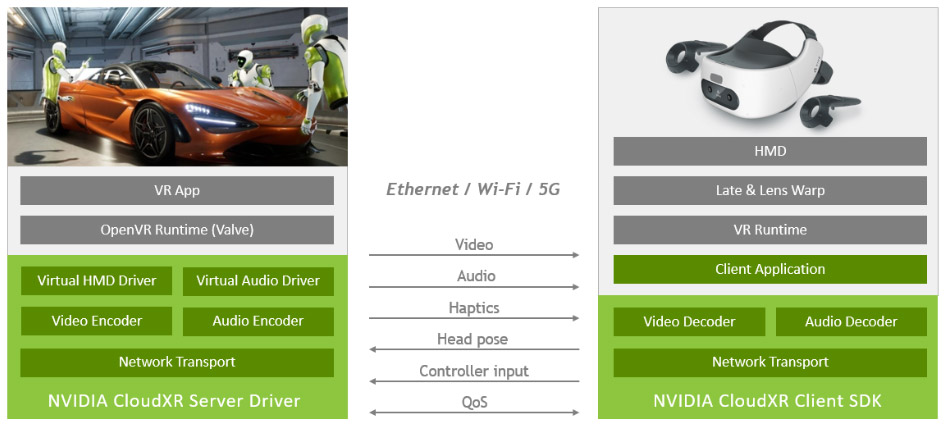
\includegraphics[scale=0.45]{nvidia-cloudxr-diagram}
\end{figure}

The CloudXR SDK from NVIDIA offers a complete solution to stream VR/AR experiences from server to client. As the only complete package in this list it is a good starting point to create a cloud \acrshort{vr} streaming prototype. After becoming familiar with the SDK the next step would be deploying it on a Server. Since Azure is the chosen cloud provider of Thales, one of the major stakeholders, it would be the first choice. \\
\newline
\begin{varwidth}[t]{.5\textwidth}
\renewcommand\labelitemi{+}
\textbf{Pros:}
\begin{itemize}
\item Only complete solution
\item Increased prototyping speed
\item Custom made for streaming \acrshort{vr} content
\item Works with cutting-edge \acrshort{gpu}'s
\end{itemize}
\end{varwidth}
\hspace{4em}
\begin{varwidth}[t]{.5\textwidth}
\renewcommand\labelitemi{-}
\textbf{Cons:}
\begin{itemize}
\item Forced to use new generation NVIDIA products (Pascal Architecture)
\item Not guaranteed to get access to solution (Have to apply to NVIDIA)
\item Limited control about the solution
\item Limited documentation about the solution, since it is brand new
\end{itemize}
\end{varwidth}

\subsubsection{WebRTC Prototype 1}
\begin{figure}[h!]
\caption{Overview of WebRTC Prototype 1}
\label{fig:pr11}
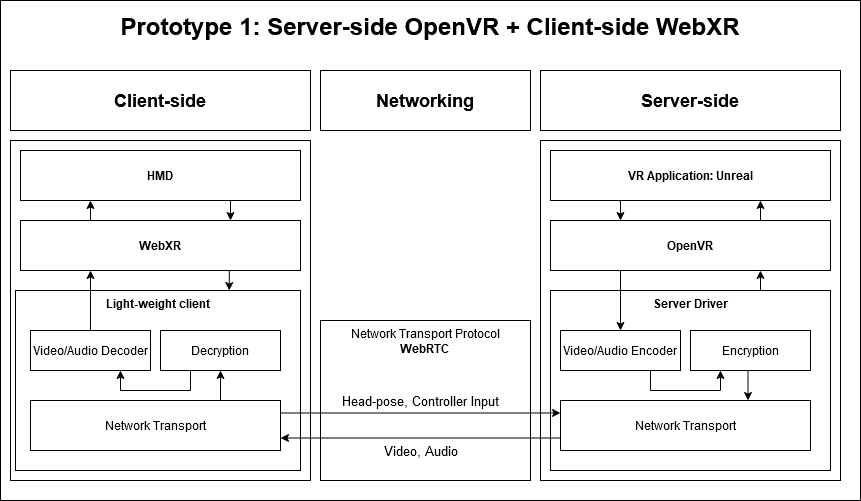
\includegraphics[scale=0.5]{CloudVR_PR1_1}
\end{figure}


WebRTC is one of the premier web technologies to enable real time communications. Since it allows for streaming video and generic data it is a good candidate to create a cloud \acrshort{vr} streaming prototype, because it can transfer both the video and input data. As it has a focus on real time communication it is optimized to reduce latency by default, however it is unclear if this is enough optimization by itself to support streaming \acrshort{vr} content. To enable the application to run "normally" OpenVR will be used to provide a virtual interface of the physical hardware on the removed remote server. By receiving pose updates from the Client and using those updates to create a virtual \acrshort{hmd} the application can be developed like a local VR application. \\
\newline
\begin{varwidth}[t]{.5\textwidth}
\renewcommand\labelitemi{+}
\textbf{Pros:}
\begin{itemize}
\item Works for the majority of \acrshort{hmd}'s and platforms
\item Mostly Open source
\item WebRTC is well documented and supported
\end{itemize}
\end{varwidth}
\hspace{4em}
\begin{varwidth}[t]{.5\textwidth}
\renewcommand\labelitemi{-}
\textbf{Cons:}
\begin{itemize}
\item Lower performance Web Technologies (but there are native clients for all major platforms available)
\item Higher complexity due to more components
\item OpenVR + WebXR are sparsely documented
\end{itemize}
\end{varwidth}

\subsubsection{WebRTC Prototype 2}
\begin{figure}[h!]
\caption{Overview of WebRTC Prototype 2}
\label{fig:pr12}
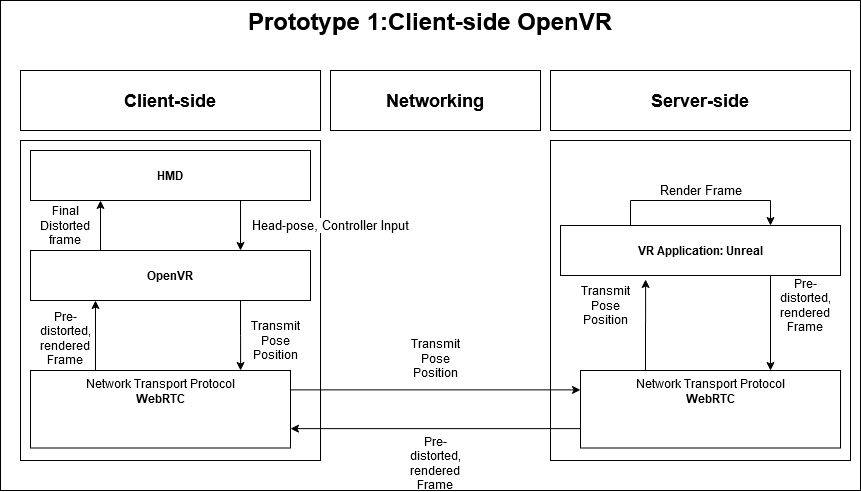
\includegraphics[scale=0.5]{CloudVR_PR1_2}
\end{figure}

This protoype candidate is similar in design to the previous one, in the sense that it uses WebRTC for networking and OpenVR for interacting with a \acrshort{hmd}. The key difference is that the application on the server does not know it is rendering specifically for VR. All the distortion operations, to generate an image for the \acrshort{hmd} from the recieved frame, will be done on the client-side with OpenVR. \\
\newline
\begin{varwidth}[t]{.5\textwidth}
\renewcommand\labelitemi{+}
\textbf{Pros:}
\begin{itemize}
\item Less complex than previous solution
\item Utilizes OpenVR to gain access to HMD's: The type/manufacturer does not matter
\end{itemize}
\end{varwidth}
\hspace{4em}
\begin{varwidth}[t]{.5\textwidth}
\renewcommand\labelitemi{-}
\textbf{Cons:}
\begin{itemize}
\item Limited usability $\rightarrow$
Not much more than a POC
\item Less sophisticated than previous solution
\end{itemize}
\end{varwidth}

\subsection{Security}

Due to a request from Thales all of the prototypes will be hosted in the Dutch Secure Defense Cloud on Microsoft Azure. Normally hosting the solution on an external server would not fulfill the security requirements, but the enivronment provided by the Dutch Secure Defense Cloud is specifically crafted for use-cases like this. It provides a physically seperated enviroment with additional security measures in compliance with the Dutch Ministry of Defence. As such most security issues are taken care of by the cloud platform.

\subsection{\acrfull{qoe}}
To measure the \acrshort{qoe} for the user, people in the XR Lab will be invited to play the prototype once it is set up. The focus is especially on users who get motion sick easily, as they provide the most valuable test data.